\subsection{Knowledge discovery: social network of avatars (virtual world)}
(Ashfaq + Vladimir)

Tasks:
\begin{itemize}
	\item Build spatio-temporal avatar profiles
	\item Group avatars into groups according to similar profiles. I.e., construct social network of profiles and do graph clustering.
	\item Predict avatar behavior from group profiles
\end{itemize}


We will use Gaussian Process dynamic models (GPDM) as profiles. GPDMs can be used for both modeling isolated avatars and interactions between avatars.  We can use a framework similar to \cite{Shen2015-jr,Shen2015-ft,Shen2012-vi}.  Then extend using our trajectory refinement and optimization approaches \cite{yoon2016}.

However, we need to consider the fact that this system is heterogeneous, i.e., things and humans.  So should have a hierarchical model, one level for things, one for humans, then merge on higher level.



Modeling the state of the cyber-human IoT avatar world is a critical component necessary for optimal IoT behavior prediction and, subsequently, decision making.  This research task focuses on novel data-driven computational models and algorithms that will enable efficient, scalable and accurate estimation of the IoT world state from a (social) network of individual IoT avatars.  In particular, we aim to solve this task by exploiting the parallel between data-driven modeling in IoT avatar worlds and modeling of complex heterogeneous crowd behaviors.


{\bf Prior Art}.  Consider the context of crowds, where the goal is not only to estimate the location of individuals in a group but also to predict group behavior, short (immediate flow) and long-term movement (e.g., crowd moving toward exit A), as well as the interaction of the crowd with the environment (e.g., residents entering of leaving an apartment).  This problem is similar to the one we are facing. However, in the IoT context, the state will not only be represented by physical spatio-temporal locations of entities but also by their general "characteristics", such as the power usage or temperature time course, etc.  Crowd state estimation may focus on macroscopic modeling (coarse flow), mesoscopic (blobs, groups of individuals), or microscopic level (individuals within a group)~\cite{zhan2008}.  Models such as the Discrete Choice~\cite{antonini2006} and the social force (SF)~\cite{helbing2005, pellegrini2009you} model were primarily designed in the context of analytics and simulation. Combining simple person sensing (tracking) with crowd modeling is essential to address the interaction of entities.  Those approaches, e.g.,\cite{bera2014,bera2015,6907095}, use crowd simulators to constrain the dynamics of measured individuals' locations by taking into account collisions.  Recent data-driven approaches~\cite{zhou2012,wang2013} aim to produce more realistic estimates of behaviors but are limited to simple environments and motion patterns and relatively short-term predictions.  Broad environments such as large residential areas, necessitate distributed models to enable sufficient coverage and efficient computation. However, no work to-date considers the detailed aspect of the joint crowd-environment state estimation in long-term planning scenarios, particularly when the states of each entity become truly multidimensional and the crowd is heterogeneous, as is the case in our social networks of IoTs.


{\bf Proposed Research}. This research focuses on the key questions of how to estimate, and subsequently predict, the joint state of the social network of IoT system.  %The estimates must yield individual states of citizens in the crowd (location, etc.), indications of physical interactions with the environment and other citizens (collisions) as well as social interactions (members of the same social group), and the ability to forecast short and long term behavior.  Because of the distributed and multimodal nature of the system, the sensor measurements will be collected and preprocessed locally and then fused to provide a comprehensive view of the system, along with the quantification of uncertainty, necessary for the subsequent stages.
We assume that the sporadic, potentially interrupted, measurements of IoT profiles, called tracklets, can be obtained from multiple sensors using existing acquisition algorithms. However, the observed tracklets will include noise and significant amount of missing information. State of the environment will be similarly measured using other static or dynamic sensors.  The state estimation will then be formulated as: {\bf Task 1: Fusion}.  Fuse and link the local measurements from multiple distributed sensors to identify correspondences between measurements of the same target process.  {\bf Task 2: IoT Crowd State Estimation}. Using the fused/linked measurements estimate the state of the IoT crowd and the environment, taking into account their social or physical interactions. {\bf Task 3: Data-driven Estimation}.  Include historical and/or simulation data to constrain and improve local and global state estimation.  To solve these Tasks we propose a global optimization framework that builds upon our preliminary work in~\cite{yoon2016}. We consider the following setup of the problem.

Consider the crowd-environment state space $\mathcal{X} = \{ ( \mathbf{T}_{i}, l_{i} ), \mathbf{Z} \}$, $\forall i \in (1, J)$  defined as the union of the set of $J$ IoT agent "trajectories" $\mathbf{T}_{i}$ and the environmental configuration $\mathbf{Z}$. The trajectories have the associated agent ID $l_{i} \in \{ 1, ... , J \}$ and temporally ordered agent states
$\mathbf{T}_{i} = \{ \mathbf{t}_{i}^{t} = (x_{i}^{t}, y_{i}^{t}) \},\quad \forall t \in (1, N_{i}),\quad x_{i}^{t}, y_{i}^{t} \in \mathbb{R},$ where $N_{i}$ denotes the number of track points available for the trajectory $i$. The environment is modeled as a set of 2D linear segments, with state $\mathbf{Z} = \{ (z_{k, x_1}^{t}, z_{k, x_2}^{t}, z_{k, y_1}^{t}, z_{k, y_2}^{t}) \},\quad \forall k=(1, N_{k}),$ where e.g., $z_{k,x_1}^{t}, z_{k,x_2}^{t}$ denote the horizontal minimum and maximum bound of the $k$-th linear obstacle at time $t$. For example, a rectangular wall is a set of four linear obstacles.  Our goal will be to reconstruct $\mathbf{T}_{i}$ and $\mathbf{Z}$ from the measurements collected by distributed IoT crowd sensors, tracklets $\mathcal{O} = \{ \mathbf{O}_i \}, i=1,\ldots,M$, and the environment sensors $\mathcal{E} = \{ \mathbf{E}_i \}, i=1,\ldots,N$. Associated with each measurement will be a quantifier of uncertainty, the measurement noise precision $u_{i}^{t}$ (e.g., supposing a Gaussian noise model). 

{\bf Task A.1 -}  We will assume that the association problem,associating each tracklet $\mathbf{O}_i$ with an agent $j \in \{ 1, ... , J \}$, need only be solved for the agents while the associations of measurements with the environment states are known and remain constant.    Typically, local sensor can produce tracklets of reasonable duration along with the profile features $\mathbf{f}_i$ describing this agent (e.g., device model, personal social profile). The linking process amounts to solving a combinatorial min-flow problem on the graph defined by tracklet compatibility costs such as the tracklet profile feature differences (e.g., $\|\mathbf{f}_i - \mathbf{f}_j\|$), spatio-temporal proximity of tracklets, etc. This is a challenging task, with approaches spanning the spectrum of exact solutions based on e.g., the Hungarian algorithm, to more tractable approximations c.f.,~\cite{tron2011b,wang2013,mazzon2013,alahi2014socially} or stochastic solutions such as JPDAF and its extensions, c.f.,~\cite{fortmann1980multi,schulz2003people}.  In this project we will first investigate solutions based on the min-flow problem formulation, which have shown reasonable performance based on our preliminary studies~\cite{yoon2016}.  We will also compare these solutions to stochastic approximations of the JPDAF type, given their ability to handle online and distributed settings~\cite{kamal2013information}.

{\bf Task A.2 -}  Given the estimated associations from Task 1, the goal here is to reconstruct $\mathbf{T}_{i}$ and $\mathbf{Z}$ from the now associated measurements $\mathbf{O}_i, i=1,\ldots,J$, and the environment sensors $\mathbf{E}_i, i=1,\ldots,N$. To illustrate our proposed approach we will focus on the specific case when the environmental configuration is known and static.  We will then first define the agent state estimation as a global multiobjective energy minimization problem.  The choice of the multiple objectives will be driven by specific and unique problem (crowd/environment) considerations.  For example, we will initially consider the following key sub-objectives, summarized in Tab.~\ref{tab:crowd_obj}:


\begin{wrapfigure}{r}{0.4\textwidth}
\vspace{-20pt}
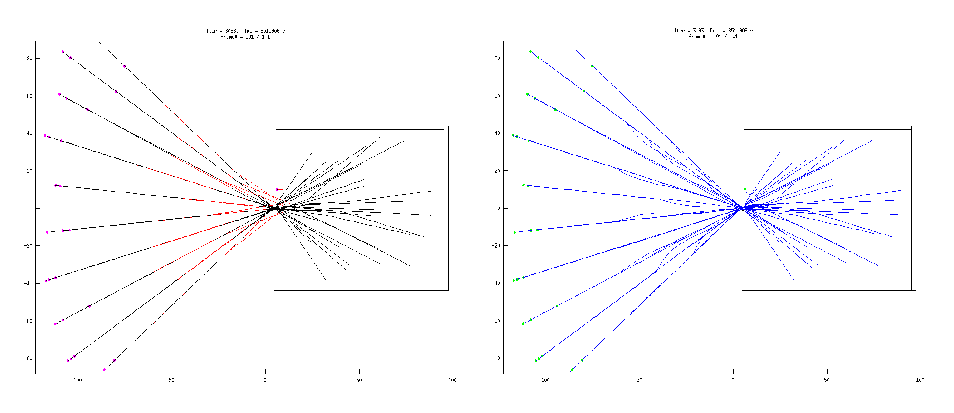
\includegraphics[width=0.38\textwidth]{wacv16_bottleneck.pdf}
\vspace{-10pt}
\caption{\small Preliminary results~\cite{yoon2016} of global microscopic trajectory refinement when 20\% of the tracklets are missing.  Black are the trajectories of 40 agents in a bottleneck benchmark simulated using the SF model, red indicate missing data, blue are refined trajectories after optimization.}
\vspace{-15pt}
\label{fig:bottleneck}
\end{wrapfigure}

\begin{table}
\centering
\caption{Multiple objective terms for global crowd-environment state estimation.}\label{tab:crowd_obj}
\tiny
\begin{tabular}{|l|l|l|l|l|} \hline
	Measurement Compatibility & Kinetic energy & Physical constraint & Social constraint & Environmental constraint \\ 
	
	$E_{gt}(\mathbf{t}_{i}^{t})$ &  
	$E_{kn}(\mathbf{t}_{i}^{t} , \mathbf{t}_{i}^{t+1})$ & 
	$E_{mv}(\mathbf{t}_{i}^{t}, \mathbf{t}_{i}^{t+1})$ &
	$C_{s}(\mathbf{t}_{i}^{t}, \mathbf{t}_{j}^{t}, \mathbf{t}_{i}^{t+1}, \mathbf{t}_{j}^{t+1}, r_{i}, r_{j})$ &
	$C_{e}(\mathbf{t}_{i}^{t}, \mathbf{t}_{i}^{t+1}, r_{i}, \mathbf{z}_{k_{1}}^{t}, \mathbf{z}_{k_{2}}^{t})$ \\ \hline
	
	$ u_{i}^{t} \| \mathbf{t}_{i}^{t} - \mathbf{o}_{i}^{t} \|^{2} $ &
	$ c_{kn} \| \mathbf{t}_{i}^{t+1} - \mathbf{t}_{i}^{t} \|^{2} $  &
	$	\begin{cases}
		0 & \text{if } \| \mathbf{t}_{i}^{t+1} - \mathbf{t}_{i}^{t} \| \le c_{mv}, \\ 
		\infty & \text{otherwise.}
		\end{cases}$ &
		
	$ \begin{cases}
		0 & \text{if } \| \alpha ( \mathbf{t}_{i}^{t+1} - \mathbf{t}_{j}^{t+1} ) + (1 - \alpha) ( \mathbf{t}_{i}^{t} - \mathbf{t}_{j}^{t} ) \|  \\
		&\quad \ge (r_{i} + r_{j}), \quad \forall \alpha \in [0, 1] \\
		\infty & \text{otherwise }
		\end{cases} $ &
	$ \begin{cases}
		0 & \text{if } \| ( \alpha \mathbf{t}_{i}^{t+1} + (1 - \alpha) \mathbf{t}_{i}^{t} ) - ( \beta \mathbf{z}_{k_{1}}^{t} + (1 - \beta) \mathbf{z}_{k_{2}}^{t} ) \|  \\
		&\quad \ge r_{i}, \quad \forall \alpha, \beta \in [0, 1] \\
		\infty & \text{otherwise }
		\end{cases} $ \\ \hline
\end{tabular}
\normalsize	
\end{table}
\emph{Compatibility with Associated Measurements}: dependency of the estimate agent trajectory on the measured tracklets; \emph{Kinetic energy}: the agents whose objective is to reach the goal position following the minimum travelled distance; \emph{Physical constraint}:  the human body set limits on the maximum walking speed $c_{mv}$ of an agent. Depending on the context, these constraints may also include the minimum speed and other biomechanical limitations, c.f.,~\cite{bento2013}; \emph{Social constraint}: Avoidance of collisions with other agents encoded through pairwise constraint functions that depend on the size of agens $r_{i}$; \emph{Environmental constraint}: Collisions between agents and the environment.


Combining the multiple objectives, our global objective will determine each track point of each $i$-th agent by solving the optimization problem
% \small
% \begin{align}
% \argmin_{ \mathbf{t}_{i}^{t} }& \sum_i \sum_{t=1}^{N_{i}} E_{gt} (\mathbf{t}_{i}^{t}) + \sum_{t=1}^{N_{i}-1} E_{kn} (\mathbf{t}_{i}^{t}, \mathbf{t}_{i}^{t+1}) + \sum_{t=1}^{N_{i}-1} E_{mv} (\mathbf{t}_{i}^{t}, \mathbf{t}_{i}^{t+1}) +\sum_{t=1}^{N_{i}} \sum_{i \neq j} C_{s}(\mathbf{t}_{i}^{t}, \mathbf{t}_{j}^{t}, \mathbf{t}_{i}^{t+1}, \mathbf{t}_{j}^{t+1}, r_{i}, r_{j})
% +\sum_{t=1}^{N_{i}} \sum_{(i,k)} C_{e}(\mathbf{t}_{i}^{t}, \mathbf{t}_{i}^{t+1}, r_{i}, \mathbf{z}_{k_{1}}^{t}, \mathbf{z}_{k_{2}}^{t}) \nonumber
% %\\
% %&+\sum_{t=2}^{N_{i}-1} E_{av} (\mathbf{t}_{i}^{t-1}, \mathbf{t}_{i}^{t}, \mathbf{t}_{i}^{t+1}, \mathbf{\tilde{t}}_{m}^{t-1}, \mathbf{\tilde{t}}_{m}^{t}, \mathbf{\tilde{t}}_{m}^{t+1})
% \end{align}
% \normalsize
%\small
%\begin{align}
$\arg\min_{ \mathbf{t}_{i}^{t} } \sum_i \sum_{t=1}^{N_{i}} E_{gt} + \sum_{t=1}^{N_{i}-1} E_{kn}$ $ + \sum_{t=1}^{N_{i}-1} E_{mv} +\sum_{t=1}^{N_{i}} \sum_{i \neq j}  $ $ +\sum_{t=1}^{N_{i}} \sum_{(i,k)} C_{e}.$
%\nonumber
%\end{align}
%\normalsize
However, direct minimization of this global objective is infeasible. In particular, collision constraints are non-convex and we desire to solve this task in a distributed manner, enabling local data processing. Additive objectives of this type are amenable to general distributed optimization using the alternating direction method of multipliers (ADMM). A particular version of that approach, investigated in~\cite{bento2013,bento2015,yoon2016}, focuses on a message-passing solution to ADMM, specifically suitable for networked sensor settings.  Here the global objective can be considered as a consensus optimization problem, where the consensus constraints stem from the need to satisfy pairwise agent-agent and agent-environment interaction "rules."  In Fig.~\ref{fig:bottleneck} we illustrate the effectiveness of this approach from our preliminary studies in~\cite{yoon2016}.  Our method is able to effectively reconstruct large portions of the missing information, while ensuring the reconstructed trajectories are without collisions and discontinuities, and still preserve the original essence of the crowd.  While this approach is appealing, its convergence may be slow (typically on order of minutes).  We will consider recent ADMM acceleration approaches particularly suitable for this setting, including our own distributed adaptive penalty Fast ADMM~\cite{song2016aaai}.  Another challenge will be to extend this point-based estimation approach to a fully probabilistic setting, with quantifiers of posterior uncertainty.  We propose to tackle this task using our recent work on ADMM for probabilistic models~\cite{yoon2012,behnam2016}, which can also be used to construct online versions of the global optimization approach.  We will compare these approaches to state-of-the-art distributed dynamical system methods, including~\cite{Das2013-mk,kamal2013information} and the recent generative-based models of~\cite{zhou2012}.

{\bf Task A.3 -}  One of the main limitations of the global optimization approaches in the limited physical and social constraints (e.g., kinetic, repulsion, etc.) that may not be fully representative of the actual IoT entity behavior.  While one can overcome these drawbacks when the tracklets are accurate and densely measured, sensor failures, etc. can result in poor state estimates.  We propose to use data-driven IoT profile priors to improve the state estimation approach.  To construct such priors we propose to use both the data from actual IoTs as well as the data simulated in our simulators.  However, such "raw" sources of data typically produce dense measurements that do not capture the "essence" of the behaviors, a desideratum for good generalization.  We thus propose to first construct summaries of behavior patterns from the raw data using methods such as dynamic trajectory clustering~\cite{johnson1996,morris2011,zhou2011,cancela2014,xu2015}.  These summaries $\mathcal{\tilde{D}} = \{ \mathbf{\tilde{T}}_{m}, \mathbf{Z} \}$ will be specific to environment configurations $\mathbf{Z}$.  Given the summaries, we will define an additional energy term $E_{av} (\mathbf{t}_{i}^{t-1}, \mathbf{t}_{i}^{t}, \mathbf{t}_{i}^{t+1}, \mathbf{\tilde{t}}_{m}^{t-1}, \mathbf{\tilde{t}}_{m}^{t}, \mathbf{\tilde{t}}_{m}^{t+1}) = \sum_m s_{m,i}^t \| \theta_{i}^{t} - \tilde{\theta}_{m}^{t} \|^{2}$ that models the compatibility of $\mathbf{t}$ with the cluster centers $\mathbf{\tilde{t}}$, where $s_{m,i}^t$ are the compatibility weights.  This energy term will be added as another subobjective to the global optimization in Task 2. Compatibility weights can be either set apriori to estimated in the optimization process (e.g., in an EM-type of recursive estimation).  We will contrast these approaches to other learning-based crowd sensing models, including~\cite{zhou2012} and~\cite{bera2015}. 

Note that all three Task possess clear dependencies.  Therefore, we will also investigate the utility of a closed-loop estimation system where the results of Task 2 and Task 3 can be used to improve the associations in Task 1.
 
%There has been several approaches to incorporate motion prior into tracker to improve accuracy~\cite{hu2008,ali2008,rodriguez2009}. Notable contributions by~\cite{pellegrini2009,eth_biwi_00785} introduce the SF model~\cite{PhysRevE.51.4282} to model the individual, dynamic social behavior in crowd. \cite{eth_biwi_01014} extended this model by proposing a multi-target tracking method that can uniformly include different types of information, e.g. appearance, physical constraints, and the social behavior of pedestrians. However, this model is not a global optimization thus an approximate inference strategy.  The works by Bera and Manocha~\cite{bera2014,bera2015} proposed a real-time iterative trajectory estimation algorithm for medium-density crowds using Kalman filters with a multi-agent motion model based on velocity obstacles~\cite{berg2008}. The key idea is to separate tracking part and waypoint estimation part, and exploit the motion model to do the latter. This framework was further extended to provide real-time, adaptive tracking for crowded scenes~\cite{6907095}.

%It should also be noted that crowd movement simulation is a complementary area to the crowd tracking, and many methods were proposed in the computer graphics community~\cite{kapadia2015virtual}. As seen in the above example prior works, crowd simulators can be used as motion priors for trackers~\cite{PhysRevE.51.4282,berg2008}. Moreover, the output of crowd trackers can be used to train data-driven crowd simulation models, e.g.~\cite{journals/cgf/LernerCL07} as obtaining large scale ground truth information for training crowd models is one of the biggest challenges~\cite{musse2010}.

%{\bf Trajectory Clustering.} Trajectory clustering is a good way to find consistent motion patterns of trajectories. It often done by iterative, unsupervised algorithms~\cite{johnson1996,zhou2011,cancela2014}. Patterns of the clusters have been described as distribution~\cite{johnson1996}, semantic path~\cite{zhou2011,zhou2012,cancela2014} or some model parameters~\cite{morris2011,hu2013}. Probabilistic approaches such as Gaussian process~\cite{ellis2009}, Gaussian mixture with Hidden Markov Models~\cite{morris2011}, Dirichlet process mixture models~\cite{hu2013} are also popular and may provide notion of uncertainty of the outcome, but they often tend to be sensitive to initialization or pre-training~\cite{morris2011}. A recently introduced method~\cite{xu2015} thus proposes a multi-kernel, mean shift based method that is less sensitive to initialization and eliminate the need of pre-defining the number of clusters. 

%{\bf Environmental constraint: Motion pattern} So far, all constraints are directly imposed on observed, input trajectories. However, there are evidences from prior work that trajectory estimated by the motion models can help tracking~\cite{bera2015}. The issue here is that the model generated trajectories in prior works (a) do not always consider environmental configuration and (b) may be too fine-grained such that it conflicts with the real world tracking results if we impose too much constraint on the model generated trajectories. Therefore, we need an interm representation on the \emph{essence} of the crowd motion given the environmental configuration.

%For this purpose, we rely on clustering. Given set of trajectories $\mathcal{\tilde{D}} = \{ \mathbf{\tilde{T}}_{m}, \mathbf{Z} \}$, each trajectory representing a cluster, i.e. motion pattern (note that the trajectories are from the same environmental configuration $\mathbf{Z}$), where $m \in \{ 1, ... , M \}$ denotes the cluster index, we consider to minimize the angular velocity between the trajectory to be refined and the most similar cluster trajectory as
% \begin{align}
% E_{av} (\mathbf{t}_{i}^{t-1}, \mathbf{t}_{i}^{t}, \mathbf{t}_{i}^{t+1}, \mathbf{\tilde{t}}_{m}^{t-1}, \mathbf{\tilde{t}}_{m}^{t}, \mathbf{\tilde{t}}_{m}^{t+1})
% 	&= \| \theta_{i}^{t} - \tilde{\theta}_{m}^{t} \|^{2}
% \end{align}
% where
% \begin{align}
% \theta_{i}^{t}
% 	&= \frac{ ( \mathbf{t}_{i}^{t} - \mathbf{t}_{i}^{t-1} ) \times ( \mathbf{t}_{i}^{t+1} - \mathbf{t}_{i}^{t} )  }{ \| \mathbf{t}_{i}^{t} - \mathbf{t}_{i}^{t-1} \|^{2} } \\
% \tilde{\theta}_{i}^{t}
% 	&= \frac{ ( \mathbf{\tilde{t}}_{m}^{t} - \mathbf{\tilde{t}}_{m}^{t-1} ) \times ( \mathbf{\tilde{t}}_{m}^{t+1} - \mathbf{\tilde{t}}_{m}^{t} )  }{ \| \mathbf{\tilde{t}}_{m}^{t} - \mathbf{\tilde{t}}_{m}^{t-1} \|^{2} }
% \end{align}
% such that
% \begin{align}
% m = \argmin_{m \in \{1, ... , M\}} \sum_{t=1}^{N_{i}} \| \mathbf{t}_{i}^{t} - \mathbf{\tilde{t}}_{m}^{t} \|^{2}.
% \end{align}
% We will discuss how to learn $\mathbf{\tilde{T}}_{m}$ clusters later.

